% \documentclass[tikz]{standalone}
\tikzset{
    level/.style = {
        ultra thick,
        black,
    },
    connect/.style = {
        dashed,
        black
    },
    notice/.style = {
        draw,
        rectangle callout,
        callout relative pointer={#1}
    },
    label/.style = {
        text width=2cm
    }
}
% \begin{document}
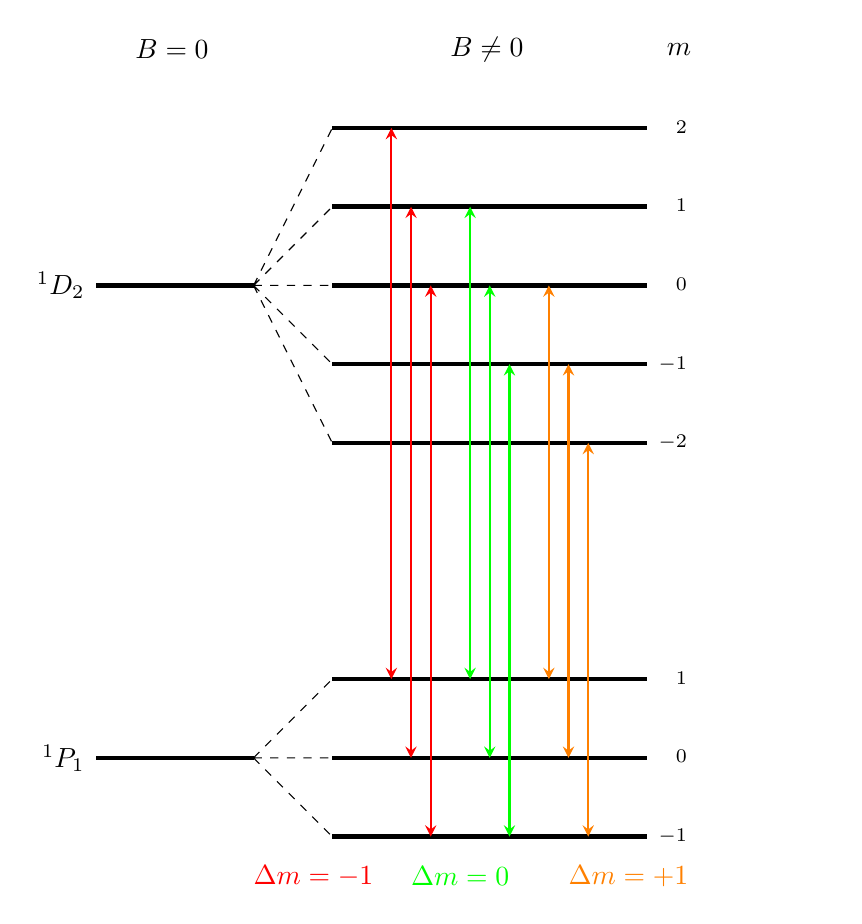
\begin{tikzpicture}
    % Draw all levels
    \draw[level] (0,+3) node[left] {$^1D_2$} -- (2,+3);
    \draw[level] (0,-3) node[left] {$^1P_1$} -- (2,-3);

    \draw[connect] (2,+3) -- (3,+5) (2,+3) -- (3,+4) (2,+3) -- (3,+3) (2,+3) -- (3,+2) (2,+3) -- (3,+1);
    \draw[connect]                  (2,-3) -- (3,-4) (2,-3) -- (3,-3) (2,-3) -- (3,-2)                 ;

    \draw[level] (3,+5) -- (7,+5) node[right] {\scriptsize $\phantom{-}2$};
    \draw[level] (3,+4) -- (7,+4) node[right] {\scriptsize $\phantom{-}1$};
    \draw[level] (3,+3) -- (7,+3) node[right] {\scriptsize $\phantom{-}0$};
    \draw[level] (3,+2) -- (7,+2) node[right] {\scriptsize $-1$};
    \draw[level] (3,+1) -- (7,+1) node[right] {\scriptsize $-2$};
    \draw[level] (3,-2) -- (7,-2) node[right] {\scriptsize $\phantom{-}1$};
    \draw[level] (3,-3) -- (7,-3) node[right] {\scriptsize $\phantom{-}0$};
    \draw[level] (3,-4) -- (7,-4) node[right] {\scriptsize $-1$};

    % Draw arrows
    \draw [stealth-stealth, thick, red]({3.5 + 1/4},+5) -- ({3.5 + 1/4},-2);
    \draw [stealth-stealth, thick, red]({3.5 + 2/4},+4) -- ({3.5 + 2/4},-3);
    \draw [stealth-stealth, thick, red]({3.5 + 3/4},+3) -- ({3.5 + 3/4},-4);
    %
    \draw [stealth-stealth, thick, green]({4.5 + 1/4},+4) -- ({4.5 + 1/4},-2);
    \draw [stealth-stealth, thick, green]({4.5 + 2/4},+3) -- ({4.5 + 2/4},-3);
    \draw [stealth-stealth, thick, green]({4.5 + 3/4},+2) -- ({4.5 + 3/4},-4);
    %
    \draw [stealth-stealth, thick, orange]({5.5 + 1/4},+3) -- ({5.5 + 1/4},-2);
    \draw [stealth-stealth, thick, orange]({5.5 + 2/4},+2) -- ({5.5 + 2/4},-3);
    \draw [stealth-stealth, thick, orange]({5.5 + 3/4},+1) -- ({5.5 + 3/4},-4);


    % Draw labels
    \node[label] at (1.5,6) {$B = 0$};
    \node[label] at (5.5,6) {$B \neq 0$};
    \node[label] at (8.25,6) {$m$};

    % \node[label, red] at ({3+0},-4.5-0) {$\mathrm\Delta m = -1$};
    % \node[label, green] at ({3+2},-4.5-0.5) {$\mathrm\Delta m = 0$};
    % \node[label, orange] at ({3+4},-4.5-1) {$\mathrm\Delta m = +1$};
    \node[label, red] at ({3+0},-4.5) {$\mathrm\Delta m = -1$};
    \node[label, green] at ({3+2},-4.5) {$\mathrm\Delta m = 0$};
    \node[label, orange] at ({3+4},-4.5) {$\mathrm\Delta m = +1$};
\end{tikzpicture}
% \end{document}
